\documentclass[10pt,twocolumn]{article}
\usepackage[margin=0.75in,columnsep=0.28in]{geometry}
\usepackage{times}
\usepackage{amsmath}
\usepackage{graphicx}
\usepackage{booktabs}
\usepackage{array}
\usepackage{tikz}
\usepackage{titlesec}
\usepackage{enumitem}
\usepackage[colorlinks=true,linkcolor=blue,citecolor=blue,urlcolor=blue]{hyperref}
\usetikzlibrary{arrows.meta,positioning}

\setlength{\parindent}{1em}
\setlength{\parskip}{0pt}

\titleformat{\section}{\normalfont\large\bfseries}{\Roman{section}.}{0.6em}{}
\titleformat{\subsection}{\normalfont\bfseries}{\Alph{subsection}.}{0.5em}{}
\titlespacing*{\section}{0pt}{8pt}{4pt}
\titlespacing*{\subsection}{0pt}{6pt}{3pt}

\begin{document}

\twocolumn[
\begin{center}
{\LARGE \bfseries Court Vision: Motion Planning for an \\ Obstacle-Aware Ball-Dribbling Mobile Robot \\[4pt]}
{\large RBE 550 Motion Planning --- Project Proposal \\[4pt]}
{\normalsize Rudy Arsenault, Tracy Yang \\
Worcester Polytechnic Institute \\[6pt]}
\end{center}
\vspace{4pt}
\hrule
\vspace{6pt}
{\small \noindent \textbf{Abstract}---We propose a mobile robot that must dribble a
ball with a paddle end-effector down a cluttered course, choosing where to
strike the ball next so that the resulting bounce location is both reachable
and collision-free. Unlike prior robot-dribbling work, which stabilizes a
periodic bounce in place, or legged locomotion work, which dribbles across
open terrain, our robot must jointly plan \emph{where the ball goes} and
\emph{where the base goes} under hard obstacle constraints, occasionally
redirecting the ball itself rather than only steering around obstacles. We
outline the hybrid dribble dynamics, the coupled interception/navigation
planner, a simulation-based validation plan in Gazebo or PyBullet, and a
week-by-week schedule with contingencies scoped to a semester-length,
sim-only team project.}
\vspace{8pt}
\hrule
\vspace{10pt}
]

\section{Introduction}
Ball dribbling is a deceptively rich motion planning problem. A player does
not simply track the ball; the player decides, on every bounce, where to
send it next, weighing the defender, the open lane, and where their own feet
need to be a half-second later.

We propose to build a simulated mobile robot with a single paddle
end-effector that must sustain a bouncing ball down a corridor cluttered
with obstacles. The robot cannot simply avoid the clutter with its base,
because the base's position is coupled to the ball's bounce location: if the
nominal next-bounce spot is blocked, the robot must instead \emph{redirect}
the ball to a different, reachable, collision-free spot, and only then plan
its base motion to intercept it there. This makes the problem a genuine
hybrid of periodic contact control (the dribble) and spatial planning under
constraints (the obstacles) with no single fixed goal configuration to plan
toward. The ``goal'' is a moving target that the robot itself is allowed to
choose within limits.

\section{Background and Related Work}
Robotic ball dribbling has been studied as a variant of robot juggling.
Bühler, Koditschek, and Kindlmann formalized juggling and catching as
intermittent dynamical tasks and introduced the ``mirror law,'' in which the
end-effector's motion is a distorted reflection of the ball's motion so that
a stable periodic bounce emerges from a simple feedback rule
\cite{buehler1994}. Bätz et al.\ showed that basketball-style dribbling can
be modeled with the same hybrid (discrete impact / continuous flight)
dynamics as juggling, and demonstrated stable multi-cycle dribbling on a
stationary industrial arm using both force/torque and vision-based ball
tracking \cite{batz2009,batz2009icra}. These works establish the dribble
controller itself, but the manipulator base never moves and there is no
notion of an obstacle to avoid.

Legged locomotion research has since pushed dribbling onto a moving
platform: DribbleBot uses reinforcement learning to let a quadruped dribble
a soccer ball across natural, uneven terrain (sand, mud, snow) while walking
\cite{dribblebot2023}. This demonstrates that dribbling and locomotion can
be coupled, but the ``obstacles'' are terrain properties that perturb the
bounce, not discrete objects that must be routed around. There is no
explicit path planning layer.

On the navigation side, classical approaches such as the dynamic window
approach \cite{fox1997} and velocity obstacles \cite{fiorini1998} plan
collision-free motion for a base among static and moving obstacles, but
they assume the robot's goal location is externally given and fixed at each
planning cycle.

Our project sits in the gap between these three bodies of work: we adopt
the hybrid dribble model of \cite{buehler1994,batz2009}, must move the base
as in \cite{dribblebot2023}, but, unlike any of the above, must also
treat the next-bounce target itself as a planning variable that can be
shifted to satisfy obstacle constraints, coupling target selection with
navigation-style path planning rather than treating them as sequential
stages.

\section{Proposed Approach}
We will simulate a differential-drive base carrying a 1-DOF vertically
actuated paddle in Gazebo or PyBullet. The ball is modeled as a sphere with
a coefficient of restitution; between contacts it follows free-fall
projectile motion, and at each paddle contact its outgoing velocity is set
by the mirror-law-style controller of \cite{buehler1994,batz2009}.

Ball state is tracked in closed loop rather than predicted from a
precomputed terrain model: after every bounce, an onboard camera estimate
of the ball's position and velocity is used to re-fit its projectile
trajectory (in the spirit of the recursive tracking used in
\cite{batz2009icra}), so that irregularities such as a tilted surface or an
imperfectly known coefficient of restitution are absorbed by
re-estimation rather than assumed away. Known obstacle geometry is used
offline to build the course's configuration-space map, but the ball's own
dynamics are always treated as sensed and re-estimated, not scripted.

The planner operates in two coupled layers, illustrated in Fig.~\ref{fig:system}:
\begin{enumerate}[nosep]
  \item \textbf{Bounce/interception layer:} given the ball's current apex
  state, predict its default landing point and time, and check that point
  against the local obstacle map (built from the course's known/perceived
  clutter, represented in configuration space as in the course's C-space
  module).
  \item \textbf{Redirect/navigation layer:} if the default landing point is
  blocked, search a small neighborhood of alternative landing points (by
  adjusting the paddle's hit angle and impulse) for one that is both
  physically reachable by the dribble controller and collision-free; then
  plan a short-horizon, collision-free base trajectory to be under that
  point in time for the next contact.
\end{enumerate}
This is the central creative and technical challenge of the project: most
motion planning projects treat ``avoid the obstacle'' and ``reach the goal''
as the whole problem, but here the robot may also negotiate with its own
target, which turns a single-shot planning query into a small per-cycle
optimization repeated at dribble frequency.

\begin{figure}[t]
\centering
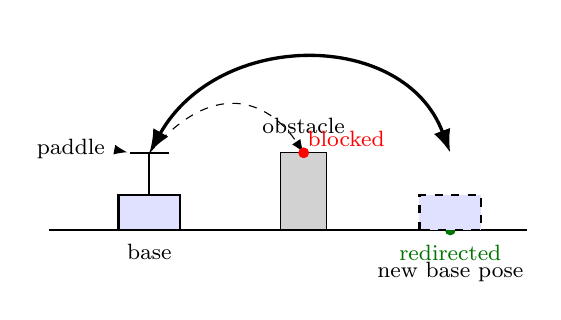
\begin{tikzpicture}[scale=0.98, every node/.style={font=\footnotesize}]
  % ground
  \draw[thick] (0,0) -- (6.2,0);
  % obstacle
  \fill[gray!35] (3.0,0) rectangle (3.6,1.0);
  \draw (3.0,0) rectangle (3.6,1.0);
  \node at (3.3,1.35) {obstacle};
  % robot base
  \draw[thick,fill=blue!12] (0.9,0) rectangle (1.7,0.45);
  \node at (1.3,-0.28) {base};
  \draw[thick] (1.3,0.45) -- (1.3,1.0);
  \draw[thick] (1.05,1.0) -- (1.55,1.0);
  \node[anchor=east] at (0.85,1.05) {paddle};
  \draw[-{Latex},shorten >=1pt] (0.95,1.02) -- (1.05,1.0);
  % nominal bounce arc (blocked by obstacle) -- stops where it hits the obstacle
  \draw[dashed,-{Latex}] (1.3,1.0) .. controls (2.2,2.05) and (2.9,1.6) .. (3.3,1.0);
  \fill[red] (3.3,1.0) circle (2pt);
  \node[red] at (3.85,1.18) {blocked};
  % redirected bounce arc
  \draw[very thick,{Latex}-{Latex}] (1.3,1.0) .. controls (2.2,2.6) and (4.6,2.6) .. (5.2,1.0);
  \fill[green!45!black] (5.2,0.0) circle (2pt);
  \node[green!45!black] at (5.2,-0.3) {redirected};
  % new base target
  \draw[thick,fill=blue!12,dashed] (4.8,0) rectangle (5.6,0.45);
  \node at (5.2,-0.55) {new base pose};
\end{tikzpicture}
\caption{The nominal next-bounce trajectory (dashed) is interrupted by an
obstacle, so the redirect layer chooses a new, reachable landing point
(solid arc) and the navigation layer re-plans the base pose to intercept it
there.}
\label{fig:system}
\end{figure}

\section{Objectives}
\begin{enumerate}[nosep]
  \item \textbf{Dribble dynamics \& controller:} implement the hybrid
  ball-paddle contact model and reproduce a stable, stationary periodic
  dribble in simulation.
  \item \textbf{Base integration:} couple the controller's commanded next
  contact point/time to a mobile-base trajectory so the robot can dribble
  while translating in an obstacle-free lane.
  \item \textbf{Static obstacle course:} build a configuration-space map of
  a course with 4--6 static obstacles and plan collision-free base paths
  that sustain the dribble through the full course.
  \item \textbf{Redirect-the-bounce planner:} when the nominal landing spot
  conflicts with an obstacle, compute an alternate hit angle/impulse that
  shifts the landing point to an open cell, and re-plan the base intercept
  accordingly, rather than only steering the base around obstacles.
  \item \textbf{Evaluation:} quantify performance versus an obstacle-free
  baseline using metrics such as dribble cycles survived, path-length
  overhead, and redirect-planner success rate across obstacle densities.
\end{enumerate}

\section{Stretch Goals}
\begin{enumerate}[nosep]
  \item \textbf{Dynamic/random clutter:} obstacles that appear or move
  during a run, requiring online re-planning rather than a single offline
  course map.
  \item \textbf{Multi-bounce lookahead:} plan two to three bounces ahead,
  similar to how a real player reads the court, instead of only the
  immediate next contact.
  \item \textbf{Physical feasibility discussion:} document what would 
  hypothetically need to change (sensing, paddle actuator bandwidth, 
  ball tracking) to carry the approach onto real hardware.
\end{enumerate}

\section{Schedule and Division of Labor}
The schedule is aligned to the official RBE 550 course calendar with
Week~8's project status update and Week~16's final report as hard
checkpoints. Week~14 is deliberately reserved as a buffer; if the
redirect-planner (Objective~4) is behind schedule at that point, the
contingency plan is to fall back to a simpler policy in which the robot
briefly catches and re-drops the ball to reset the bounce phase whenever
the nominal target is blocked, rather than shifting the hit angle, which is a
strictly easier version of the same idea that still produces a working,
demonstrable system.

\begin{table}[h]
\centering
\small
\setlength{\tabcolsep}{4pt}
\begin{tabular}{@{}>{\raggedright\arraybackslash}p{1.05cm}p{6.35cm}@{}}
\toprule
\textbf{Wk} & \textbf{Objectives} \\
\midrule
3 & Submit proposal; finalize team roles; stand up sim environment; deep-read dribbling/juggling and obstacle-avoidance literature. \\
\mbox{4--5} & Implement ball-paddle contact model and mirror-law-style controller; validate stationary periodic dribble (Obj.~1). \\
\mbox{6--7} & Attach base and couple contact point to base trajectory; build C-space map for a static obstacle course; first collision-free dribble-and-drive runs (Obj.~2--3). \\
8 & \textbf{Project status update}: demonstrate baseline dribble + static-obstacle navigation. \\
\mbox{9--10} & Design and implement redirect-the-bounce planner; begin extending to moving obstacles (Obj.~4). \\
\mbox{11--12} & Robustness passes; failure-mode testing; metrics/logging pipeline (Obj.~5). \\
13 & Full evaluation sweep across obstacle densities; begin stretch goals if ahead of schedule. \\
14 & \textbf{Buffer week} / contingency fallback if needed (see above). \\
15 & Finalize results and demo video; begin final report. \\
16 & \textbf{Final report and presentation due.} \\
\bottomrule
\end{tabular}
\end{table}

\noindent\textbf{Division of labor:} Yang will own the dribble dynamics,
contact controller, and ball state estimation (Obj.~1, part of Obj.~4);
Arsenault will own the configuration-space obstacle mapping, base path
planning, and simulation/evaluation infrastructure (Obj.~2--3, Obj.~5).
Both members will jointly design and implement the redirect-the-bounce
planner (Obj.~4), since coupling the two halves of the system is the core
intellectual contribution of the project, and will co-write the final
report.

\section{Expected Results}
We expect a simulation demo showing the robot sustaining a dribble through
a static obstacle course that a purely base-avoidance planner (one that
never adjusts the ball's landing spot) cannot complete without dropping the
ball or stalling. We will report, as a function of obstacle density, the
dribble-survival rate, the extra path length incurred by redirect events
versus the obstacle-free baseline, and qualitative video comparisons. If
stretch goals are reached, we will additionally report performance under
randomly moving clutter and with multi-bounce lookahead.

\begin{thebibliography}{9}
\bibitem{buehler1994} M.~Bühler, D.~E. Koditschek, and P.~J. Kindlmann,
``Planning and control of robotic juggling and catching tasks,''
\emph{The International Journal of Robotics Research}, vol.~13, no.~2,
pp.~101--118, 1994.

\bibitem{batz2009} G.~Bätz, M.~Sobotka, D.~Wollherr, and M.~Buss, ``Robot
basketball: Ball dribbling -- a modified juggling task,'' in \emph{Advances
in Robotics Research}, T.~Kröger and F.~M. Wahl, Eds. Berlin, Heidelberg:
Springer, 2009, pp.~323--334.

\bibitem{batz2009icra} G.~Bätz, K.-K. Lee, D.~Wollherr, and M.~Buss, ``Robot
basketball: A comparison of ball dribbling with visual and force/torque
feedback,'' in \emph{Proc.\ IEEE Int.\ Conf.\ on Robotics and Automation
(ICRA)}, 2009.

\bibitem{dribblebot2023} Y.~Ji, G.~B. Margolis, and P.~Agrawal, ``DribbleBot:
Dynamic legged manipulation in the wild,'' in \emph{Proc.\ IEEE Int.\ Conf.\
on Robotics and Automation (ICRA)}, 2023.

\bibitem{fox1997} D.~Fox, W.~Burgard, and S.~Thrun, ``The dynamic window
approach to collision avoidance,'' \emph{IEEE Robotics \& Automation
Magazine}, vol.~4, no.~1, pp.~23--33, 1997.

\bibitem{fiorini1998} P.~Fiorini and Z.~Shiller, ``Motion planning in
dynamic environments using velocity obstacles,'' \emph{The International
Journal of Robotics Research}, vol.~17, no.~7, pp.~760--772, 1998.
\end{thebibliography}

\end{document}